\documentclass[12pt]{beamer}
\usepackage{../Estilos/BeamerFC}
\usepackage{../Estilos/ColoresLatex}
\usepackage{courier}
\usepackage{listingsutf8}
\usepackage{listings}
\usepackage{xcolor}
\usepackage{textcomp}
\usepackage{color}
\definecolor{deepblue}{rgb}{0,0,0.5}
\definecolor{brown}{rgb}{0.59, 0.29, 0.0}
\definecolor{OliveGreen}{rgb}{0,0.25,0}
% \usepackage{minted}

\DeclareCaptionFont{white}{\color{white}}
\DeclareCaptionFormat{listing}{\colorbox{gray}{\parbox{0.98\textwidth}{#1#2#3}}}
\captionsetup[lstlisting]{format=listing,labelfont=white,textfont=white}
\renewcommand{\lstlistingname}{Código}


\definecolor{Code}{rgb}{0,0,0}
\definecolor{Keywords}{rgb}{255,0,0}
\definecolor{Strings}{rgb}{255,0,255}
\definecolor{Comments}{rgb}{0,0,255}
\definecolor{Numbers}{rgb}{255,128,0}

\makeatletter

\newif\iffirstchar\firstchartrue
\newif\ifstartedbyadigit
\newif\ifprecededbyequalsign

\newcommand\processletter
{%
  \ifnum\lst@mode=\lst@Pmode%
    \iffirstchar%
        \global\startedbyadigitfalse%
      \fi
      \global\firstcharfalse%
    \fi
}

\newcommand\processdigit
{%
  \ifnum\lst@mode=\lst@Pmode%
      \iffirstchar%
        \global\startedbyadigittrue%
      \fi
      \global\firstcharfalse%
  \fi
}

\lst@AddToHook{OutputOther}%
{%
  \lst@IfLastOtherOneOf{=}
    {\global\precededbyequalsigntrue}
    {}%
}

\lst@AddToHook{Output}%
{%
  \ifprecededbyequalsign%
      \ifstartedbyadigit%
        \def\lst@thestyle{\color{orange}}%
      \fi
    \fi
  \global\firstchartrue%
  \global\startedbyadigitfalse%
  \global\precededbyequalsignfalse%
}

\lstset{ 
language=Python,                % choose the language of the code
basicstyle=\footnotesize\ttfamily,       % the size of the fonts that are used for the code
numbers=left,                   % where to put the line-numbers
numberstyle=\scriptsize,      % the size of the fonts that are used for the line-numbers
stepnumber=1,                   % the step between two line-numbers. If it is 1 each line will be numbered
numbersep=5pt,                  % how far the line-numbers are from the code
backgroundcolor=\color{white},  % choose the background color. You must add \usepackage{color}
showspaces=false,               % show spaces adding particular underscores
showstringspaces=false,         % underline spaces within strings
showtabs=false,                 % show tabs within strings adding particular underscores
frame=single,   		% adds a frame around the code
tabsize=2,  		% sets default tabsize to 2 spaces
captionpos=t,   		% sets the caption-position to bottom
breaklines=true,    	% sets automatic line breaking
breakatwhitespace=false,    % sets if automatic breaks should only happen at whitespace
escapeinside={| |},  % if you want to add a comment within your code
stringstyle =\color{OliveGreen},
otherkeywords={as, np.array, np.concatenate, np.linspace, linspace, interpolate.interp1d, kind, plt.plot, .copy, np.arange, np.cos, np.pi, lw, ls, label, splrep, splev, plt.legend, loc, plt.title, plt.ylim, plt.show, sign, math.ceil, math.log, np.sqrt, np.exp, np.zeros, plt.xlabel, plt.ylabel, plt.xlim, np.identity, random, np.dot, np.outer, np.diagonal },             % Add keywords here
keywordstyle = \color{blue},
commentstyle = \color{darkcerulean},
identifierstyle = \color{black},
literate=%
         {á}{{\'a}}1
         {é}{{\'e}}1
         {í}{{\'i}}1
         {ó}{{\'o}}1
         {ú}{{\'u}}1
%
%keywordstyle=\ttb\color{deepblue}
%fancyvrb = true,
}

\lstdefinestyle{FormattedNumber}{%
    literate={0}{{\textcolor{red}{0}}}{1}%
             {1}{{\textcolor{red}{1}}}{1}%
             {2}{{\textcolor{red}{2}}}{1}%
             {3}{{\textcolor{red}{3}}}{1}%
             {4}{{\textcolor{red}{4}}}{1}%
             {5}{{\textcolor{red}{5}}}{1}%
             {6}{{\textcolor{red}{6}}}{1}%
             {7}{{\textcolor{red}{7}}}{1}%
             {8}{{\textcolor{red}{8}}}{1}%
             {9}{{\textcolor{red}{9}}}{1}%
             {.0}{{\textcolor{red}{.0}}}{2}% Following is to ensure that only periods
             {.1}{{\textcolor{red}{.1}}}{2}% followed by a digit are changed.
             {.2}{{\textcolor{red}{.2}}}{2}%
             {.3}{{\textcolor{red}{.3}}}{2}%
             {.4}{{\textcolor{red}{.4}}}{2}%
             {.5}{{\textcolor{red}{.5}}}{2}%
             {.6}{{\textcolor{red}{.6}}}{2}%
             {.7}{{\textcolor{red}{.7}}}{2}%
             {.8}{{\textcolor{red}{.8}}}{2}%
             {.9}{{\textcolor{red}{.9}}}{2}%
             {\ }{{ }}{1}% handle the space
         ,%
          %mathescape=true
          escapeinside={__}
          }



\usetheme{Warsaw}
\usecolortheme{seahorse}
%\useoutertheme{default}
\setbeamercovered{invisible}
% or whatever (possibly just delete it)
\setbeamertemplate{section in toc}[sections numbered]
\setbeamertemplate{subsection in toc}[subsections numbered]
\setbeamertemplate{subsection in toc}{\leavevmode\leftskip=3.2em\rlap{\hskip-2em\inserttocsectionnumber.\inserttocsubsectionnumber}\inserttocsubsection\par}
\setbeamercolor{section in toc}{fg=blue}
\setbeamercolor{subsection in toc}{fg=blue}
\setbeamercolor{frametitle}{fg=blue}
\setbeamertemplate{caption}[numbered]

\setbeamertemplate{footline}
\beamertemplatenavigationsymbolsempty
\setbeamertemplate{headline}{}


\makeatletter
\setbeamercolor{section in foot}{bg=gray!30, fg=black!90!orange}
\setbeamercolor{subsection in foot}{bg=blue!30}
\setbeamercolor{date in foot}{bg=black}
\setbeamertemplate{footline}
{
  \leavevmode%
  \hbox{%
  \begin{beamercolorbox}[wd=.333333\paperwidth,ht=2.25ex,dp=1ex,center]{section in foot}%
    \usebeamerfont{section in foot} \insertsection
  \end{beamercolorbox}%
  \begin{beamercolorbox}[wd=.333333\paperwidth,ht=2.25ex,dp=1ex,center]{subsection in foot}%
    \usebeamerfont{subsection in foot}  \insertsubsection
  \end{beamercolorbox}%
  \begin{beamercolorbox}[wd=.333333\paperwidth,ht=2.25ex,dp=1ex,right]{date in head/foot}%
    \usebeamerfont{date in head/foot} \insertshortdate{} \hspace*{2em}
    \insertframenumber{} / \inserttotalframenumber \hspace*{2ex} 
  \end{beamercolorbox}}%
  \vskip0pt%
}
\makeatother

\makeatletter
\patchcmd{\beamer@sectionintoc}{\vskip1.5em}{\vskip0.8em}{}{}
\makeatother

%\newlength{\depthofsumsign}
%\setlength{\depthofsumsign}{\depthof{$\sum$}}
% \newcommand{\nsum}[1][1.4]{% only for \displaystyle
%     \mathop{%
%         \raisebox
%             {-#1\depthofsumsign+1\depthofsumsign}
%             {\scalebox
%                 {#1}
%                 {$\displaystyle\sum$}%
%             }
%     }
% }
\def\scaleint#1{\vcenter{\hbox{\scaleto[3ex]{\displaystyle\int}{#1}}}}
\def\scaleoint#1{\vcenter{\hbox{\scaleto[3ex]{\displaystyle\oint}{#1}}}}
\def\bs{\mkern-12mu}

\usefonttheme{serif}

\title{\large{Tema 1 - Errores y artimética de punto flotante}}
\author{M. en C. Gustavo Contreras Mayén}
\date{ }

\begin{document}
\maketitle

\section*{Contenido}
\frame[allowframebreaks]{\frametitle{Contenido} \tableofcontents[currentsection, hideallsubsections]}

\section{Más sobre los errores}
\frame{\tableofcontents[currentsection, hideothersubsections]}
\subsection{Fuentes de error}
\begin{frame}
\frametitle{Hablando de errores}
El problema es que como científicos, queremos un resultado correcto o al menos en el que la incertidumbre sea pequeña y de tamaño conocido.
\end{frame}
\begin{frame}
\frametitle{Fuentes de errores computacionales}
Existen al menos cuatro fuentes de errores que se pueden presentar en los cálculos computacionales:
\pause
\setbeamercolor{item projected}{bg=asparagus,fg=arsenic}
\setbeamertemplate{enumerate items}{%
\usebeamercolor[bg]{item projected}%
\raisebox{1.5pt}{\colorbox{bg}{\color{fg}\footnotesize\insertenumlabel}}%
}
\begin{enumerate}[<+->]
\item Un modelo equivocado.
\item Errores aleatorios.
\item Errores por aproximación
\item Errores por redondeo.
\end{enumerate}
\end{frame}

\subsection{Errores aleatorios}

\begin{frame}
\frametitle{Errores aleatorios}
Se presenta una imprecisión debida por acontecimientos tales como: fluctuaciones en la electrónica, incidencia de rayos cósmicos, o alguien que se tropieza con un enchufe.
\\
\bigskip
\pause
Éstos errores pueden ser raros, pero no tenemos ningún control sobre ellos y su probabilidad aumenta conforme transcurre el tiempo.
\end{frame}

\subsection{Errores por aproximación}

\begin{frame}
\frametitle{Errores por aproximación}
La imprecisión surge de la simplificación de las matemáticas para que un problema pueda ser resuelto en la computadora.
\\
\bigskip
\pause
Incluyen la sustitución de series infinitas por sumas finitas, intervalos infinitesimales por finitos, y funciones variables por constantes.
\end{frame}
\begin{frame}
\frametitle{Errores por aproximación}
Por ejemplo:
\pause
\begin{eqnarray}
\begin{aligned}[b]
\sin(x) &= \nsum_{n = 1}^{\infty} \: \dfrac{(-1)^{n-1} \: x^{2n - 1}}{(2n - 1)!} \hspace{0.5cm} \text{(exacta)} \\[5pt] \pause
& \simeq \nsum_{n = 1}^{N} \: \dfrac{(-1)^{n-1} \: x^{2n - 1}}{(2n - 1)!} \hspace{0.5cm} \text{(aproximación)} \pause \\[5pt] \pause
& = \sin(x) + \varepsilon(x, N)
\end{aligned}
\label{eq:ecuacion_02_02}
\end{eqnarray}
\pause
donde $\varepsilon(x,N)$ es el error por la aproximación, en este caso $\varepsilon$ corresponde a los términos desde $N + 1$ a $\infty$.
\end{frame}
\begin{frame}
\frametitle{Errores por aproximación}
Dado que el error por la aproximación se genera en el algoritmo que usamos para aproximar la matemática, también se le conoce como \underline{error del algoritmo}.
\end{frame}
\begin{frame}
\frametitle{Errores por aproximación}
Para una buena y razonable aproximación, el error debido por la aproximación debería de reducirse cuando el valor de $N$ se incrementa, y debería de anularse en el límite $N \rightarrow \infty$.
\end{frame}
\begin{frame}
\frametitle{Errores por aproximación}
Para el ejemplo (\ref{eq:ecuacion_02_02}), como la escala de $N$ se fija por el valor de $x$, un pequeño error de aproximación requiere que $ N \geqslant x$.
\\
\bigskip
\pause
Por lo que si $x$ y $N$ son valores cercanos entre sí, el error de aproximación será grande.
\end{frame}

\subsection{Errores por redondeo}

\begin{frame}
\frametitle{Errores por redondeo}
La imprecisión se genera por el número finito de dígitos utilizados para almacenar números de punto flotante.
\\
\bigskip
\pause
Estos \enquote{errores} son análogos a la incertidumbre en la medición de una cantidad física encontrada en un laboratorio de física.
\end{frame}
\begin{frame}
\frametitle{Errores por redondeo}
El error general de redondeo se acumula a medida que el equipo maneja más números, es decir, a medida que aumenta el número de pasos en un cálculo, y puede hacer que algunos algoritmos se vuelvan inestables con un rápido aumento del error.
\end{frame}
\begin{frame}
\frametitle{Errores por redondeo}
En algunos casos, el error por redondeo puede convertirse en el componente principal en la respuesta, lo que lleva a lo que los expertos informáticos llaman \azulfuerte{basura}.
\end{frame}
\begin{frame}
\frametitle{Errores por redondeo}
Por ejemplo, si la computadora mantiene cuatro decimales, entonces almacenará $\frac{1}{3}$ como $0.3333$ y $\frac{2}{3} = 0.6667$, donde el equipo ha \enquote{redondeado} el último dígito en $\dfrac{2}{3}$.
\end{frame}
\begin{frame}
\frametitle{Errores por redondeo}
Por consiguiente, si hacemos en la computadora un cálculo tan simple como $2 \frac{1}{3} - \frac{2}{3}$, produce:
\pause
\begin{equation}
2 \left( \dfrac{1}{3} \right) - \dfrac{2}{3} = 0.6666 - 0.6667 = -0.0001 \neq 0
\label{eq:ecuacion_02_03}
\end{equation}
\pause
Aunque el resultado es pequeño, no es $0$, y si se repite este cálculo varios millones de veces, \pause la respuesta final puede que ni siquiera sea pequeña (\textcolor{lava}{la basura genera basura}).
\end{frame}

\section{Modelos para el desastre}
\frame{\tableofcontents[currentsection, hideothersubsections]}
\subsection{Definiciones}

\begin{frame}[fragile]
\frametitle{Definiciones}
Sea $x$ el valor exacto de una cierta cantidad y $x^{*}$ la aproximación a esa cantidad.
\\
\bigskip
\pause
Por definición, el valor absoluto asociado a $x$ es:
\pause
\begin{equation}
\Delta = \abs{ x - x^{*} } 
\label{eq:ecuacion_01_03}	
\end{equation}
\end{frame}
\begin{frame}
\frametitle{Definiciones}
En general, los cálculos numéricos operan con aproximaciones tanto a las cantidades como a sus errores absolutos.
\\
\bigskip
\pause
En el caso ideal, en el que, además de la aproximación $x$, también se conocería el error absoluto exacto, el número exacto sería exactamente expresable como:
\pause
\begin{equation}
x = x^{*} \pm \Delta^{*}
\label{eq:ecuacion_01_04}    	
\end{equation}    
\end{frame}
\begin{frame}
\frametitle{Definiciones}
Sin embargo, en general, solo está disponible una estimación del error absoluto y, en consecuencia, solo un estimado del valor exacto puede determinarse:
\pause
\begin{equation}
x^{*} - \Delta \leq x \leq x^{*} + \Delta
\label{eq:ecuacion_01_05}
\end{equation}
\end{frame}
\begin{frame}
\frametitle{Definiciones}
Para que la estimación $x^{*}$ sea confiable, es importante que $\Delta$ no subestime el error verdadero, es decir, $\Delta \geq \Delta^{*}$, en este caso, se denomina \emph{limitación de error absoluto}.
\end{frame}
\begin{frame}
\frametitle{Más definiciones}
El error relativo $\delta^{*}$ es la aproximación de $x^{*}$ a $x$, y es igual al cociente del error absoluto con el número exacto:
\pause
\begin{equation}
\delta^{*} = \dfrac{\Delta^{*}}{\abs{x}} \hspace{1cm} x \neq 0
\label{eq:ecuacion_01_06}
\end{equation}
\end{frame}
\begin{frame}
\frametitle{Más definiciones}
Re-emplazando $\Delta^{*}$ en la ecuación(\ref{eq:ecuacion_01_04}) de la ecuación (\ref{eq:ecuacion_01_06}), tendremos la expresión para un número exacto:
\pause
\begin{equation}
x \simeq x^{*} \: (1 \pm \delta^{*})
\label{eq:ecuacion_01_07}
\end{equation}
\end{frame}
\begin{frame}
\frametitle{Más definiciones}
Basándose en el error relativo de la aproximación $\delta \geq \delta^{*}$, se expresa el valor exacto como:
\begin{equation}
x \simeq x^{*} \: (1 \pm \delta)
\label{eq:ecuacion_01_08}
\end{equation}
\end{frame}

\section{Errores en las op. aritméticas}
\frame{\tableofcontents[currentsection, hideothersubsections]}
\subsection{Errores en las op. elementales}

\begin{frame}
\frametitle{Errores en las operaciones elementales}
Revisaremos la forma en que varias operaciones elementales propagan los errores relativos de sus operandos.
\\
\bigskip
\pause
En relación con los cálculos numéricos, las consideraciones desarrolladas a continuación se refieren específicamente a los errores de redondeo y truncamiento.
\end{frame}

\subsection{Error en la suma}

\begin{frame}
\frametitle{Error en la suma}
Sea la suma de dos números próximos, $x_{1}$ y $x_{2}$, que tienen el mismo signo.
\\
\bigskip
\pause
La suma evidentemente conserva el signo y acumula las magnitudes de los operandos:
\pause
\begin{equation}
x = x_{1} + x_{2}
\label{eq:ecuacion_01_14}
\end{equation}
\end{frame}
\begin{frame}
\frametitle{Error en la suma}
Tenemos que el error total es:
\begin{align*}
\Delta x =  \Delta x_{1} + \Delta x_{2}
\end{align*}
\pause
pero, dado que los errores individuales pueden, en función de sus signos, compensarse mutuamente y acumularse.
\end{frame}
\begin{frame}
\frametitle{Error en la suma}
La suma de los errores absolutos de los operandos proporciona en realidad un límite superior para el error absoluto total de la suma:
\begin{equation}
\Delta \leq \Delta_{1} + \Delta_{2}
\label{eq:ecuacion_01_15}
\end{equation}
\end{frame}
\begin{frame}
\frametitle{Error relativo en la suma}
El error relativo de la suma de dos números proximos del mismo signo no supera el error relativo más grande de los sumandos:
\pause
\begin{equation}
\delta \leq \max{(\delta_{1}, \delta_{2})}
\label{eq:ecuacion_01_16}
\end{equation}
\end{frame}

\subsection{Error en la diferencia}

\begin{frame}
\frametitle{Error en la diferencia}
Ahora consideremos la diferencia de dos números próximos con \emph{el mismo signo}:
\pause
\begin{equation}
x = x_{1} - x_{2}
\label{eq:ecuacion_01_18}
\end{equation}
\pause
Debería ser evidente que las ecuaciones (\ref{eq:ecuacion_01_14}) y (\ref{eq:ecuacion_01_18}) cubren todas las posibles situaciones algebraicas.
\end{frame}
\begin{frame}
\frametitle{Error en la diferencia}
Al igual que en el caso de la suma, el caso más desfavorable es aquél en el que los errores absolutos se potencian entre sí, y, por lo tanto, la suma de los errores absolutos es, de nuevo, el límite superior para el error absoluto de la diferencia:
\pause
\begin{align*}
\Delta \leq  \Delta_{1} + \Delta_{2}
\end{align*}
\end{frame}
\begin{frame}
\frametitle{Error en la diferencia}
Maximizando el error absoluto total en la definición de error relativo ($\delta$), tenemos que:
\pause
\begin{equation}
\delta \leq \dfrac{\Delta_{1} + \Delta_{2}}{\abs{x_{1} - x_{2}}} = \dfrac{\abs{x_{1}} \: \delta_{1} + \abs{x_{2}} \: \delta_{2}}{\abs{x_{1} - x_{2}}}
\end{equation}
\end{frame}
\begin{frame}
\frametitle{Error en la diferencia}
Si los sumandos están cerca de su valor, la diferencia absoluta $\abs{x_{1} - x_{2}}$ es pequeño e, incluso para pequeños errores relativos individuales, $\delta_{1}$ y $\delta_{2}$, el error relativo de la diferencia, $\delta$, puede volverse significativo.
\end{frame}

\subsection{Error en el producto}

\begin{frame}
\frametitle{Error en el producto}
El error relativo de un producto de dos números próximos $x = x_{1} \: x_{2}$, no excede a la suma del error relativo de los factores $\delta_{1}$ y $\delta_{2}$:
\pause
\begin{equation}
\delta = \delta_{1} + \delta_{2}
\label{eq:ecuacion_01_20}
\end{equation}
\end{frame}

\subsection{Error en el cociente}

\begin{frame}
\frametitle{Error en el cociente}
Consideremos ahora el cociente:
\begin{align*}
x = \dfrac{x_{1}}{x_{2}}
\end{align*}
de dos números próximos no nulos.
\\
\bigskip
\pause
Teniendo en cuenta, una vez más, que $x_{1}$ y $x_{2}$ se ven afectados por pequeños errores absolutos $\Delta_{1} = \abs{\Delta x_{1}}$ y $\Delta_{2} = \abs{\Delta x_{2}}$:
\end{frame}
\begin{frame}
\frametitle{Error en el cociente}
Obtenemos la relación límite:
\pause
\begin{equation}
\delta = \delta_{1} + \delta_{2}
\label{eq:ecuacion_01_27}
\end{equation}
que establece que el error relativo del cociente no excede los errores relativos acumulados del dividendo y divisor.
\end{frame}

\section{Ejercicios}
\frame{\tableofcontents[currentsection, hideothersubsections]}
\subsection{Aproximando con una serie}

\begin{frame}
\frametitle{Retomando el problema}
Veamos el resultado y su error al hacer una aproximación de la expresión:
\pause
\begin{align*}
\sin(x) \simeq \nsum_{n = 1}^{N} \: \dfrac{(-1)^{n-1} \: x^{2n-1}}{(2 \, n - 1)!}
\end{align*}
\end{frame}
\begin{frame}
\frametitle{Punto importante}
No perdamos de vista que la anterior expresión nos indica que debemos de calcular $(-1)^{n-1} \: x^{2n-1}$, \pause para luego dividirlo entre $(2 \, n - 1)!$.
\\
\bigskip
\pause
No es una buena idea para implementarla en el código.
\end{frame}
\begin{frame}
\frametitle{Punto importante}
Para valores grandes de $n$:
\setbeamercolor{item projected}{bg=bananayellow,fg=bistre}
\setbeamertemplate{enumerate items}{%
\usebeamercolor[bg]{item projected}%
\raisebox{1.5pt}{\colorbox{bg}{\color{fg}\footnotesize\insertenumlabel}}%
}
\begin{enumerate}[<+->]
\item Calcular el factorial puede consumir demasiado tiempo.
\item Elevar a la potencia, puede causar un \textcolor{ao}{overflow}, y como es el denominador, no queremos problemas en esta parte.
\end{enumerate}
\end{frame}
\begin{frame}
\frametitle{Cambiando el cálculo}
Cambiemos la operación de la siguiente manera: \pause usaremos una multiplicación que nos relacione el \emph{\textcolor{blue-violet}{siguiente término}} con un \emph{\textcolor{burgundy}{término previo}} de la serie.
\end{frame}
\begin{frame}
\frametitle{Relación entre los términos}
\begin{eqnarray*}
\begin{aligned}
\dfrac{(-1)^{n-1} \, x^{2n-1}}{(2 \, n - 1)!} &= \dfrac{-x^{2}}{(2 \, n - 1)(2 \, n -2)} \, \dfrac{(-1)^{n-2} \, x^{2n-3}}{(2 \, n - 3)!} \\[1em] \pause
\Rightarrow \hspace{0.2cm} n \, \text{término} &= \dfrac{-x^{2}}{(2 \, n - 1)(2 \, n -2)} \, (n - 1) \, \text{término}
\end{aligned}
\end{eqnarray*}
\end{frame}
\begin{frame}
\frametitle{Primera propuesta de código}
Implementemos una primera propuesta de código, que luego de revisarla tendrá una mejora.
\end{frame}
\begin{frame}
\frametitle{¿Qué es lo que hará el código?}
Debemos de introducir un valor $x$ de tal manera que se evalúe con la suma finita, toma en cuenta que la función \funcionazul{math.sin(x)}, el argumento $x$ debe de estar en radianes.
\\
\bigskip
\pause
Podemos hacer la conversión conocida de la geometría, \pause o utilizar la función \funcionazul{math.radians(x)} para obtener el valor en radianes.
\end{frame}
\begin{frame}
\frametitle{¿Qué es lo que hará el código?}
Luego vamos a calcular el error relativo (con una función de usuario), ocupando como valor \enquote{exacto} el que nos devuelve la función \funcionazul{math.sin(x)} de \python.
\\
\bigskip
\pause
Usemos el valor de $x = \SI{30}{\degree}$ para el ejercicio.
\end{frame}
\begin{frame}[allowframebreaks, fragile]
\frametitle{Primera propuesta de código}
\begin{lstlisting}[caption=Código para aproximar sen(x)]
import math

# Aqui va la funcion para el error relativo
# def funcion(arg1, arg2):
#     codigo necesario


a = float(input('Teclea el valor a evaluar: '))
x = math.radians(a)

j = 0
n = 10
suma = x
term =  x

print('x \t exacta \t   suma \t  error')
for i in range(2, n):
    j += 1
    term = (-term *x*x)/((2*i-1)*(2*i-2))
    suma  = suma + term
    print('{0:} \t {1:1.10f} \t {2:1.5e}'.format(j, suma, error(arg1, arg2)))
\end{lstlisting}
\end{frame}
\begin{frame}
\frametitle{Resultado}
\begin{table}
\renewcommand{\arraystretch}{0.8}
\begin{tabular}{c c c}
Iteración & Aproximación & Error \\ \hline
$1$ & $0.4996741794$ & $6.51641e-02$ \\
$2$ & $0.5000021326$ & $4.26518e-04$ \\
$3$ & $0.4999999919$ & $1.62620e-06$ \\
$4$ & $0.5000000000$ & $4.05599e-09$ \\
$5$ & $0.5000000000$ & $7.12763e-12$ \\
$6$ & $0.5000000000$ & $1.11022e-14$ \\
$7$ & $0.5000000000$ & $0.00000e+00$ \\
$8$ & $0.5000000000$ & $0.00000e+00$ \\
\end{tabular}
\end{table}
\end{frame}

% \section{Errores en las funciones esféricas de Bessel}
% \frame[allowframebreaks]{\tableofcontents[currentsection, hideothersubsections]}
% \subsection{Funciones de Bessel}
% \begin{frame}
% \frametitle{Funciones de Bessel}
% La acumulación de errores por redondeo a menudo limita la capacidad de un programa para calcular con precisión.
% \\
% \bigskip
% \pause
% Revisaremos como ejercicio, la manera de calcular las funciones esféricas de Bessel $j_{\ell}(x)$ y de Neumann $n_{\ell}(x)$.
% \end{frame}
% \begin{frame}
% \frametitle{Funciones de Bessel}
% Estas funciones son respectivamente, las soluciones regulares/irregulares (no singulares / singulares en el origen) de la ecuación diferencial
% \begin{equation}
% x^{2} \: f^{\prime \prime} (x) + 2 \: x \: f^{\prime}(x) + [ x^{2} - \ell ( \ell + 1)] \: f(x) = 0
% \label{eq:ecuacion_02_19}
% \end{equation}
% \end{frame}
% \begin{frame}
% \frametitle{Funciones de Bessel y esféricas de Bessel}
% Las funciones esféricas de Bessel se relacionan con las funciones de Bessel de primera clase por
% \[ j_{\ell}(x) = \sqrt{\dfrac{\pi}{2 \: x}} \: J_{n + \frac{1}{2}} (x) \]
% \end{frame}
% \begin{frame}
% \frametitle{Funciones de Bessel y esféricas de Bessel}
% Se encuentran en diversos problemas de la física, como la expansión de una onda plana en ondas esféricas parciales
% \begin{equation}
% e^{i \: \mathbf{k \cdot r}} = \sum_{\ell = 0}^{\infty} i^{\ell} \: (2 \: \ell + 1) \: j_{\ell} (k \:  r) \: P_{\ell}(\cos \theta)
% \label{eq:ecuacion_02_20}
% \end{equation}    
% \end{frame}
% \begin{frame}
% \frametitle{Funciones esféricas de Bessel de orden $n$}
% \fontsize{12}{12}\selectfont
% A continuación se muestra una gráfica con las funciones esféricas de Bessel de orden $n = 0, \ldots, 5$:
% \begin{figure}
% \centering
% 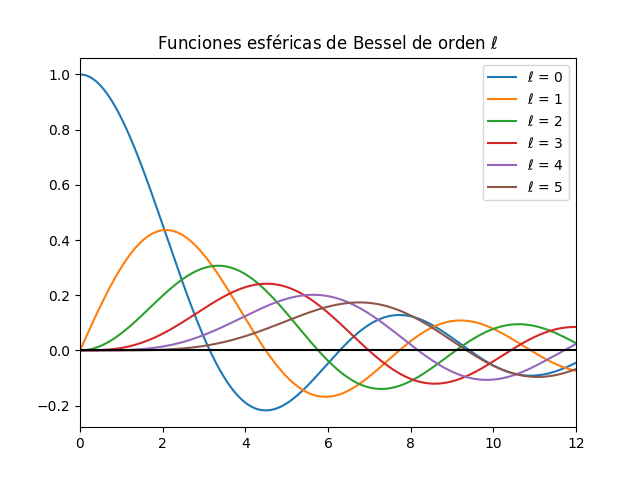
\includegraphics[scale=0.4]{funcionesEsfericasBessel}
% \caption{La gráfica se generó usando la librería de funciones especiales de \python.}
% %\caption{Nótese que para valores pequeños de $x$, los valores para un $\ell$ mayor, se hacen prograsivamente más pequeños.}
% \end{figure}
% \end{frame}
% \begin{frame}
% \frametitle{Valores para $\ell = 0, 1$}
% Los dos primero valores para $\ell$ son
% \begin{align}
% j_{0} (x) &= + \dfrac{\sin x}{x}, \hspace{1cm} j_{1} (x) = +\dfrac{\sin x}{x^{2}} - \dfrac{\cos x}{x} \label{eq:ecuacion_02_21} \\
% &{} \nonumber \\
% n_{0} (x) &= - \dfrac{\cos x}{x}, \hspace{1cm} n_{1} (x) = -\dfrac{\cos x}{x^{2}} - \dfrac{\sin x}{x} \label{eq:ecuacion_02_22}
% \end{align}
% \end{frame}
% \subsection{Ejercicio: Relaciones de recursión}
% \begin{frame}
% \frametitle{Relaciones de recursión}
% La manera clásica de calcular las funciones de Bessel de orden $j$: $j_{\ell} (x)$ es sumar su serie de potencias para valores pequeños de $\frac{x}{\ell}$ y sumando su expansión asintótica para valores de $x$ grandes.
% \end{frame}
% \begin{frame}
% \frametitle{Relaciones de recurrencia}
% El enfoque que usaremos, se basa en \emph{las relaciones de recurrencia}:
% \begin{align}
% j_{\ell + 1} (x) = \dfrac{2 \: \ell + 1}{x} \: j_{\ell}(x) - j_{\ell - 1}(x) \hspace{0.5cm} \mbox{hacia arriba} \label{eq:ecuacion_02_23}  \\
% {} \nonumber \\ 
% j_{\ell - 1} (x) = \dfrac{2 \: \ell + 1}{x} \: j_{\ell}(x) - j_{\ell + 1}(x) \hspace{0.5cm} \mbox{hacia abajo} \label{eq:ecuacion_02_24}
% \end{align}
% \end{frame}
% \begin{frame}
% \frametitle{Relaciones de recurrencia}
% Las ecuaciones (\ref{eq:ecuacion_02_23}) y (\ref{eq:ecuacion_02_24}) son la misma relación:
% \setbeamercolor{item projected}{bg=blue!70!black,fg=yellow}
% \setbeamertemplate{enumerate items}[circle]
% \begin{enumerate}[<+->]
% \item Una escrita para la recurrencia hacia adelante que parte de valores pequeños a valores grandes de $\ell$.
% \item La otra relación de recurrencia es descendente para valores de $\ell$ pequeños.
% \end{enumerate}
% \pause
%  Con unas cuantas sumas y multiplicaciones, las relaciones de recurrencia permiten el cálculo rápido y sencillo de todo el conjunto de valores de $j_{\ell}$ para $x$ fijo y todo $\ell$.
% \end{frame}
% \begin{frame}
% \frametitle{Relaciones de recurrencia}
% Para la relación de recurrencia hacia adelante de $\ell$ para un $x$ fijo, comenzamos con las formas conocidas para $j_{0}$ y $j_{1}$ (\ref{eq:ecuacion_02_21}) y usamos (\ref{eq:ecuacion_02_23}).
% \end{frame}
% \begin{frame}
% \frametitle{Relaciones de recurrencia}
% Como veremos, esta recurrencia hacia adelante parece funcionar al principio, pero luego falla.
% \\
% \bigskip
% La razón de la falla se puede ver en las gráficas de $j_{\ell}(x)$ y $n_{\ell}(x)$ como función de $x$.
% \end{frame}
% \begin{frame}
% \frametitle{Relaciones de recurrencia}
% \begin{figure}
% \centering
% 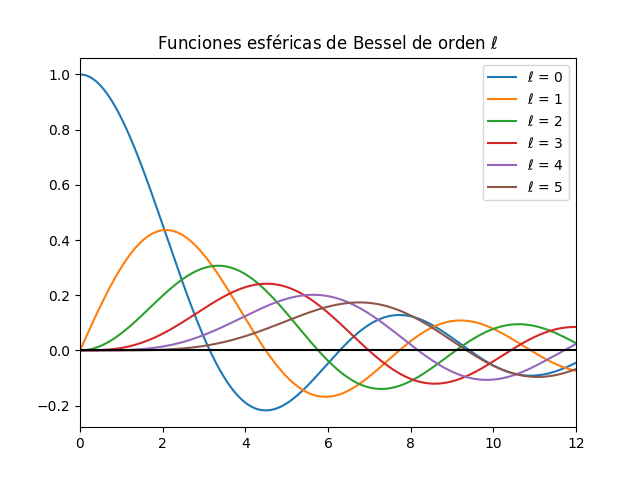
\includegraphics[scale=0.5]{funcionesEsfericasBessel}
% \end{figure}
% \end{frame}
% \begin{frame}
% \frametitle{Relaciones de recurrencia}
%  Si iniciamos con  $x \simeq 2$ y $\ell = 0$, veremos que a medida que la  recurrencia hacia adelante para  $j_{\ell}$ con valores mayores de $\ell$ con (\ref{eq:ecuacion_02_23}), esencialmente tomamos la diferencia de dos funciones \enquote{grandes} para producir un valor \enquote{pequeño} para $j_{\ell}$.
% \end{frame}
% \begin{frame}
% \frametitle{Relaciones de recurrencia}
% Este proceso sufre de cancelación sustractiva y siempre reduce la precisión.
% \\
% \bigskip
% A medida que continuamos con la recurrencia, tomamos la diferencia de dos funciones pequeñas con errores grandes y producimos una función más pequeña con un error aún mayor. Después de cierto tiempo, nos quedamos con sólo el error de redondeo (basura).
% \end{frame}
% \begin{frame}
% \frametitle{Estimando el error}
% Para ser más específicos, llamemos $j_{\ell}^{(c)}$ al valor numérico que calculamos como nua aproximación para $j_{\ell}(x)$.
% \\
% \bigskip
% Por lo que si comenzamos con un valor neto $j_{\ell}$, después de un corto tiempo la falta de precisión de la computadora se mezcla efectivamente en un poco de $n_{\ell}$:
% \begin{equation}
% j_{\ell}^{(c)} = j_{\ell} (x) + \varepsilon \: n_{\ell} (x)
% \label{eq:ecuacion_02_25}	
% \end{equation}
% \end{frame}
% \begin{frame}
% \frametitle{Estimando el error}
% Esto no lo podemos evitar, porque tanto $j_{\ell}$ como $n_{\ell}$ satisfacen la misma ecuación diferencial y, por esa razón, la misma relación de recurrencia.
% \\
% \bigskip
% La mezcla de $n_{\ell}$ se convierte en un problema cuando el valor numérico de $n_{\ell}(x)$ es mucho mayor que el de $j_{\ell} (x)$ porque incluso una cantidad minúscula de un número muy grande puede ser grande.
% \end{frame}
% \begin{frame}
% \frametitle{Estimando el error}
% Por el contrario, si usamos la relación de recurrencia hacia adelante (\ref{eq:ecuacion_02_23}) para generar la función esférica de Neumann $n_{\ell}$, no habrá ningún problema porque estamos combinando funciones pequeñas para producir más grandes, ya que es un proceso que no contiene cancelación sustractiva.
% \end{frame}
% \begin{frame}
% \frametitle{Solución al problema}
% La solución simple a este problema es usar (\ref{eq:ecuacion_02_24}) para la recursión descendente de los valores de $j_{\ell}$ que comienzan en un valor grande $\ell = L$.
% \\
% \bigskip
% Esto evita la cancelación sustractiva tomando valores pequeños de $j_{\ell + 1} (x)$ y $j_{\ell}(x)$ y generando por la suma un valor mayor en $j_{\ell -1}(x)$.
% \end{frame}
% \begin{frame}
% \frametitle{Solución al problema}
% Mientras que el error todavía puede mantenerse como una función de Neumann, la magnitud real del error disminuirá rápidamente conforme la recurrencia hacia atrás use valores pequeños de $\ell$.
% \end{frame}
% \begin{frame}
% \frametitle{Solución al problema}
% De hecho, si empezamos iterando hacia atrás con valores arbitrarios para $j_{L + 1}^{(x)}$ y $j_{L}^{(c)}$, después de un corto tiempo llegaremos a la correcta relación de $\ell$ para este valor de $x$.
% \end{frame}
% \begin{frame}
% \frametitle{Solución al problema}
% Aunque el valor numérico de $j_{0}^{c}$ así obtenido no será correcto porque depende de los valores arbitrarios asumidos para $j_{L + 1}$ y $j_{L}^{(c)}$, los valores relativos serán precisos. 
% \end{frame}
% \begin{frame}
% \frametitle{Solución al problema}
% Los valores absolutos se fijan a partir del valor conocido (\ref{eq:ecuacion_02_21}), $j_{0} (x) = \sin x / x$.
% \\
% \bigskip
% Debido a que la relación de recurrencia es una relación lineal entre los valores de $j_{\ell}$, sólo necesitamos normalizar todos los valores calculados mediante 
% \end{frame}
% \begin{frame}
% \frametitle{Solución al problema}
% \begin{equation}
% j_{\ell}^{\text{normalizada}} = j_{\ell}^{(c)} (x) \times \dfrac{j_{0}^{\text{analitica}}}{j_{0}^{(c)}}
% \label{eq:ecuacion_02_26}
% \end{equation}
% En consecuencia, después de haber terminado la recurrencia hacia abajo, se obtendrá la respuesta final normalizando todos los valores de $j_{\ell}^{(c)}$ basados en el valor conocido para $j_{0}$.
% \end{frame}
% \begin{frame}[fragile]
% \frametitle{Propuesta de código}
% Veamos la manera de implementar un código con \python para calcular el valor de la función esférica de Bessel con la recurrencia hacia atrás.
% \end{frame}
% \begin{frame}[allowframebreaks, fragile]
% \frametitle{Propuesta de código}
% \begin{lstlisting}[caption=Usando la regla de recurrencia hacia atrás, style= FormattedNumber, basicstyle=\linespread{0.9}\ttfamily\small, columns=fullflexible]
% import numpy as np
% import matplotlib.pyplot as plt
% import scipy.special as spl

% Xmax = 40.
% Xmin = 0.25
% paso = 0.1
% orden = 10
% inicio = 50

% def abajo (x, n, m):
%      j = np.zeros( (inicio + 2), float)
%      j[m+_1_] = j[m] = 1.
     
%      for k in range(m, 0, -1):
%          j[k-_1_] = ((2.*k + 1.)/x)*j[k] - j[k+_1_]
     
%      escala = (np.sin(x)/x)/j[0]
     
%      return j[n] * escala

% valoresy = []

% valoresx = []

% for x in np.arange(Xmin, Xmax, paso):
%     valoresy.append(abajo(x, orden, inicio))
%     valoresx.append(x)

% plt.plot(valores_x, valores_y, color='r')
% plt.axhline(y=0, ls='dashed', color = 'k')
% plt.xlim([0.25, 40])
% plt.show()
% \end{lstlisting}
% \end{frame}
% \begin{frame}
% \frametitle{Función aproximada}
% \begin{figure}
% \centering
% 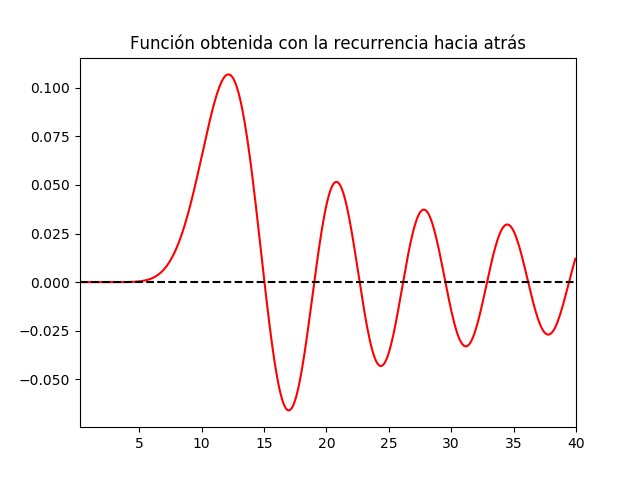
\includegraphics[scale=0.5]{funcionesEsfericasBessel_02}
% \caption{Gráfica obtenida con el algoritmo propuesto}
% \end{figure}
% \end{frame}
\end{document}